\subsection{Klassediagram og metodebeskrivelse}
Ud fra implementeringen er der genereret illustrerende klassediagrammer som kan ses på figur \ref{fig:GUI_KD}, disse klasser ligger under Libary, som kan ses på figur \ref{fig:web}, klasserne er anvendt til at kunne oprette objekter, både ud fra indholdet i databasen og til at lave en Socket klient. Hvis der ønskes yderligere indsigt i hvordan specifik kode er skrevet henvises der til sourcekoden\footnote{Se bilag under Software\textbackslash www\textbackslash lib}.

\begin{figure}[H]
    \centering
    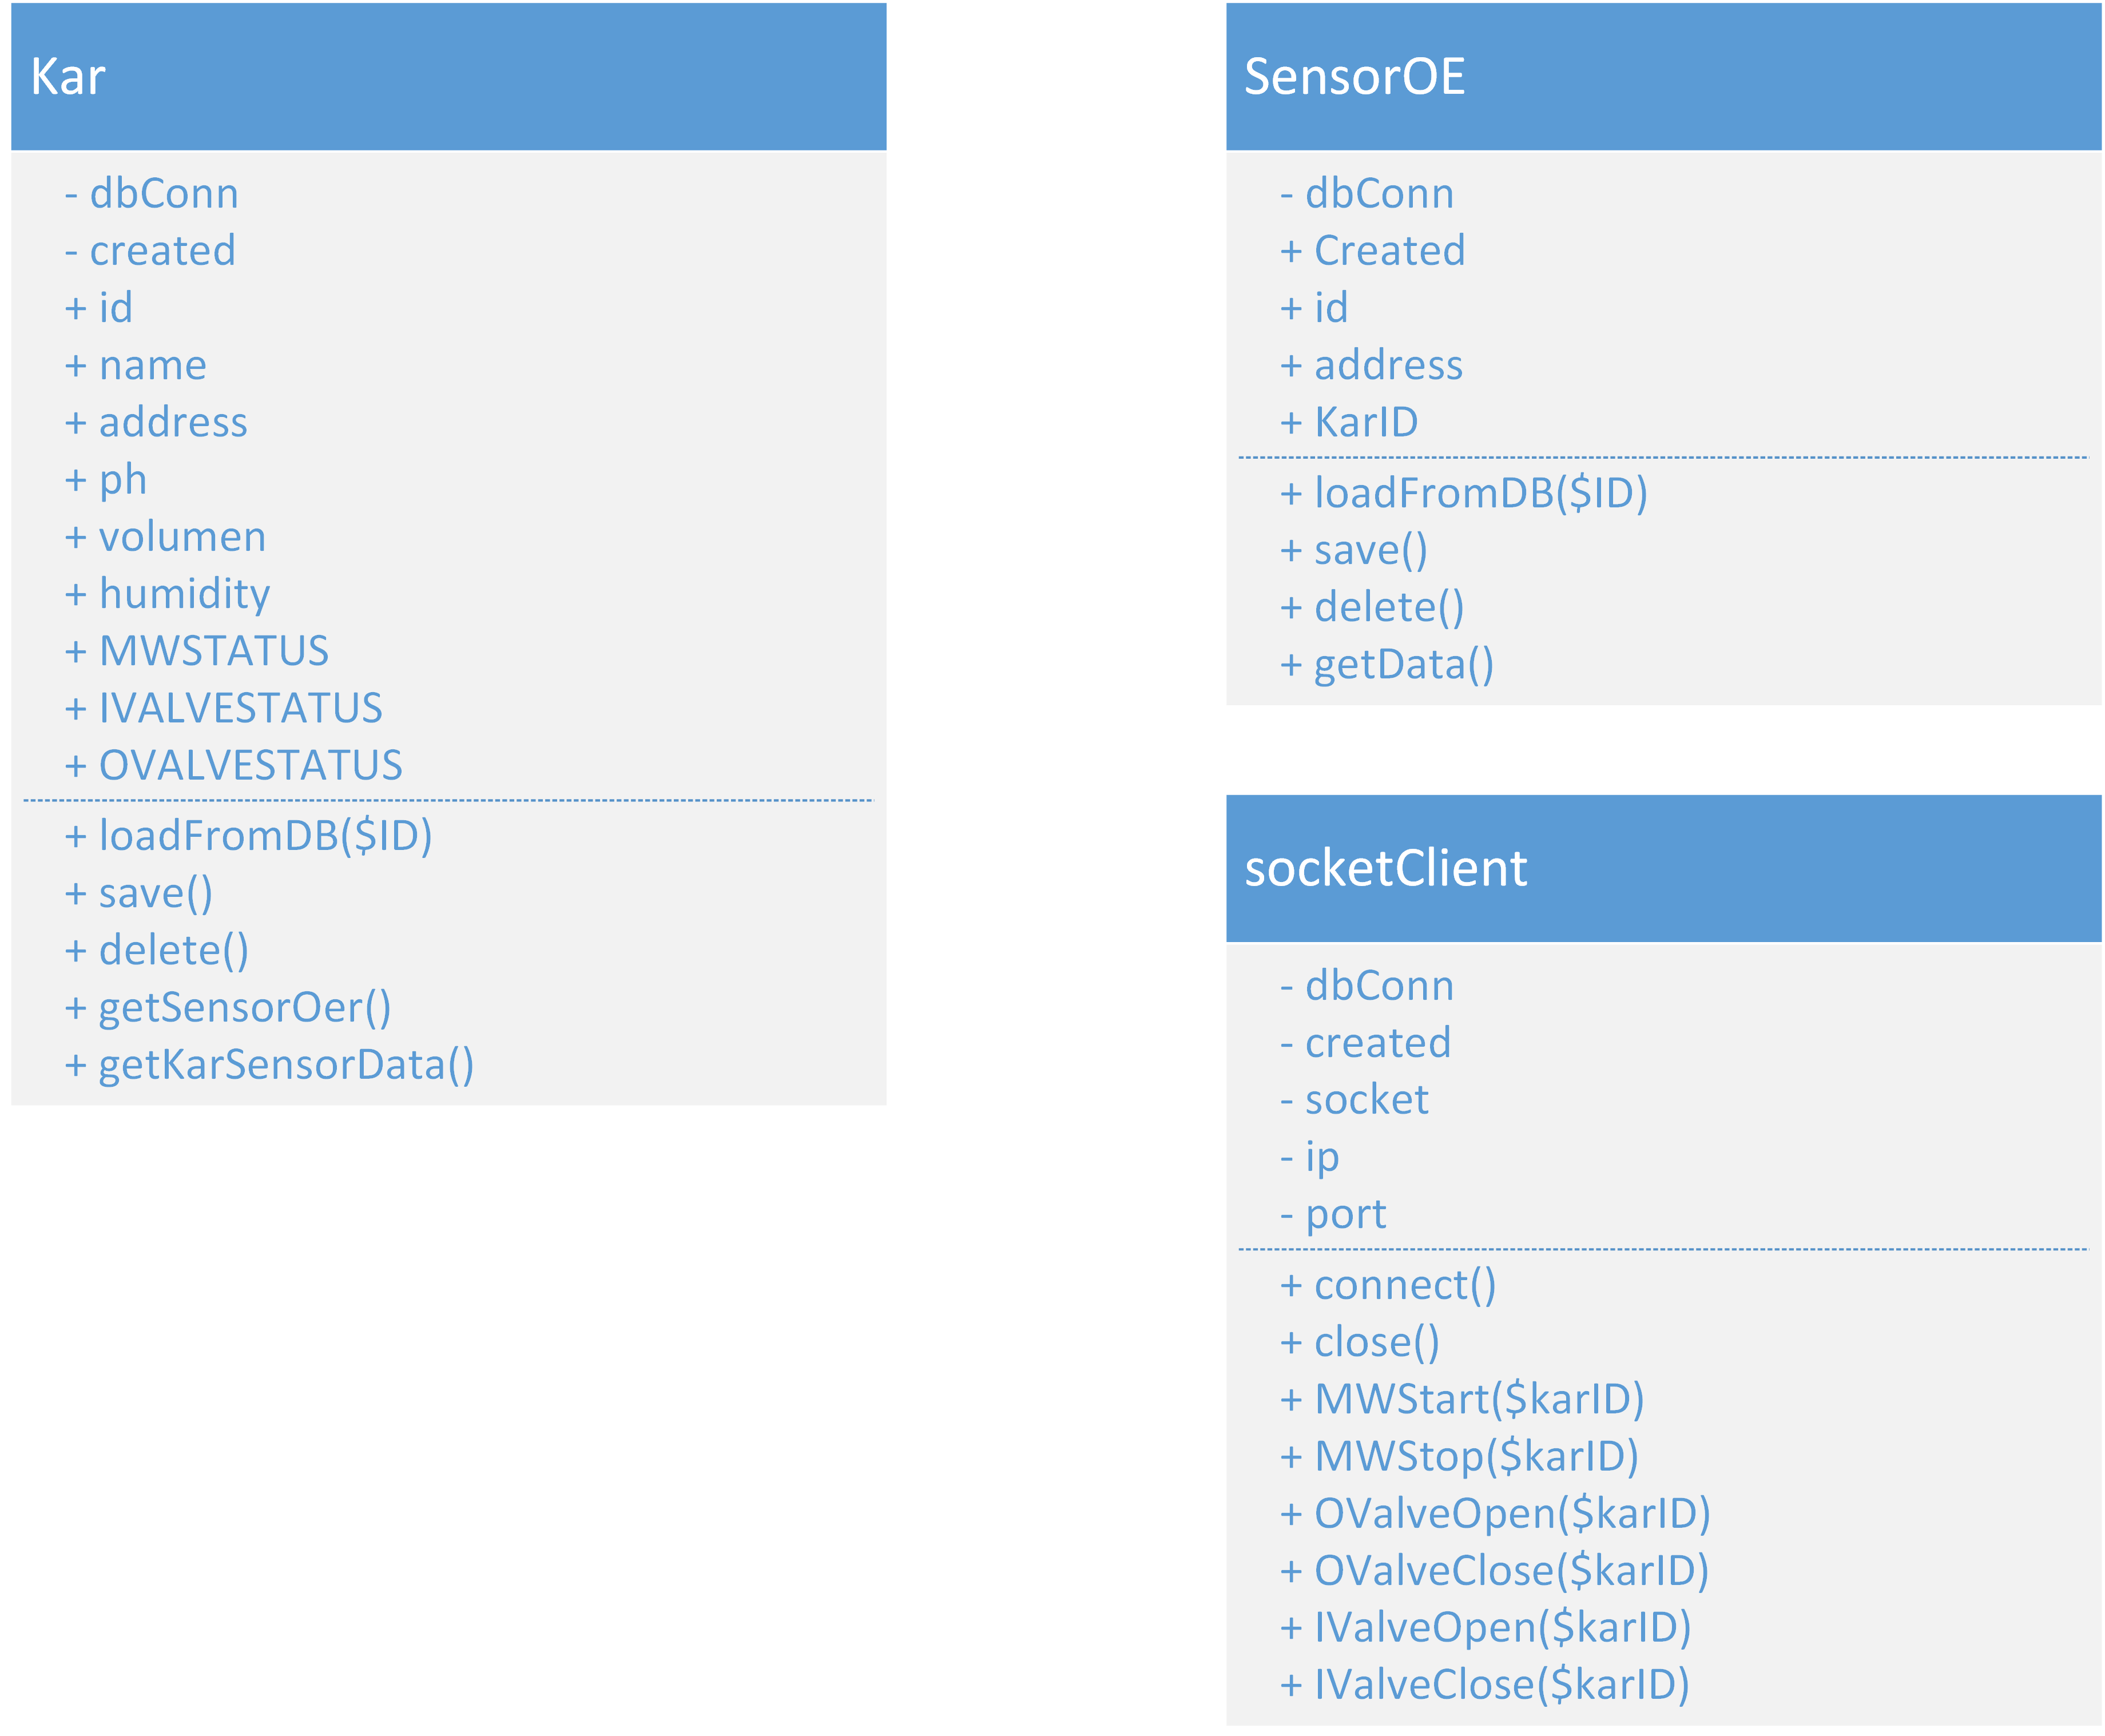
\includegraphics[width=0.9\textwidth]{SoftwareArkitektur/GUI/KlasseDiagram/photo/klasseDiagram_gui.PNG}
    \caption{Klassediagram for GUI}
    \label{fig:GUI_KD}
\end{figure}

Her kan man se der ikke er nogle forbindelse mellem de tre klasser, og det skyldes at de får alt deres information om de andre klasser gennem databasen.
 
\subsubsection{Kar klassen}
Kar klassen er en klasse, der giver mulighed for at tilgå et kar fra databasen og få alt dens information baseret på dens id, dvs. man kan oprette et kar som et objekt. Via klassens metoder kan de forskellige data i databasen blive redigeret, karet kan blive oprettet/slettet og man kan se hvilke \glslink{sensoroe}{Sensor Øer} der sider på karet. Den har følgende metoder:

\funk{public function loadFromDB(\$ID)}
{Funktionen loader alle data fra et kar i databasen med tilhørende \$ID, og sætter attributterne}
{bool}
{
\funkArg{\$ID}{Karets unikke id}
}

\funk{public function save()}
{Indsætter eller opdaterer data i databasen, alt efter om kar er oprettet}
{ingen}

\funk{public function delete()}
{Sletter karet og dets data fra databasen}
{ingen}

\funk{public function getSensorOer()}
{Opretter et array af alle Sensor Øer der sider på tilhørende kar, dette gør den ud fra databasen}
{Et array af Sensorøer}

\funk{public function getKarSensorData()}
{opretter et array af den nyeste af hver type sensor der sider på karet og deres målinger, dette gør den ud fra databasen}
{Et array at sensor type og deres målinger}


Uden for klassen er der yderligere lavet en funktion til at hente alle kar

\funk{function getKars(\$conn)}
{opretter et array af alle kar, dette gør den ud fra databasen}
{Et array af alle kar}
{
\funkArg{\$conn}{Et objekt der repræsenterer forbindelsen til databasen}
}

\subsubsection{SensorOe klassen}
SensorOe klassen er en klasse, der giver mulighed for tilgå en Sensor Ø fra databasen og få alt dens information baseret på dens id, dvs. man kan oprette et kar som et objekt. Via klassens metoder kan de forskellige data i databasen blive redigeret, Sensor Øen kan blive oprettet/slettet og man kan se hvilket kar Sensir Øen tilhører. Den har følgende metoder:

\funk{public function loadFromDB(\$ID)}
{Funktionen loader alle data fra en Sensor Ø i databasen med tilhørende \$ID, og sætter attributterne}
{bool}
{
\funkArg{\$ID}{Sensor Øens unikke id}
}

\funk{public function save()}
{Indsætter eller opdaterer data i databasen, alt efter om Sensor Øen er oprettet}
{ingen}

\funk{public function delete()}
{Sletter Sletter Sensor Øen og dets data fra databasen}
{ingen}

\funk{public function getData()}
{opretter et array af den nyeste af hver type sensor der sider på Sensor Øen og deres målinger, dette gør den ud fra databasen}
{Et array at sensor type og deres målinger}


\subsubsection{SocketClient klassen}
SocketClient klassen er en socket klient der anvendes til at sende beskeder direkte til FlexPMS, for at give besked om nogle ting systemet skal gøre. Den har følgende metoder:

\funk{public function connect()}
{Opretter en socket og forbinder den til serveren}
{ingen}

\funk{public function close()}
{Lukker for socket}
{ingen}

\funk{public function MWStart(\$karID)}
{Ventilerne til Sensor Øerne åbnes og manuel vanding starter}
{ingen}
{
\funkArg{\$ID}{id'et på karet}
}

\funk{public function MWStop(\$karID)}
{Ventilerne til Sensor Øerne lukkes og manuel vanding stopper}
{ingen}
{
\funkArg{\$ID}{id'et på karet}
}

\funk{public function IValveOpen(\$karID)}
{Sender en string til serveren at indløbsventilen skal åbnes}
{ingen}
{
\funkArg{\$ID}{id'et på indløbsventilens kar}
}

\funk{public function IValveClose(\$karID)}
{Sender en string til serveren at indløbsventilen skal lukkes}
{ingen}
{
\funkArg{\$ID}{id'et på indløbsventilens kar}
}

\funk{public function OValveOpen(\$karID)}
{Sender en string til serveren at afløbsventilen skal åbnes}
{ingen}
{
\funkArg{\$ID}{id'et på afløbsventilens kar}
}

\funk{public function OValveClose(\$karID)}
{Sender en string til serveren at afløbsventilen skal lukkes}
{ingen}
{
\funkArg{\$ID}{id'et på afløbsventilens kar}
}

\funk{public function AddSonsorOe(\$karID, \$SOeID)}
{Funktionen sender en besked om hvilken Sensor Ø der er blevet tilføjet, baseret på dens id og det kars id, som den sider på}
{ingen}
{
\funkArg{\$karID}{id'et på karet}
\funkArg{\$SOeID}{id'et på Sensor Øen}
}


\funk{public function DeleteSonsorOe(\$karID, \$SOeID)}
{Funktionen sender en besked om hvilken Sensor Ø der er blevet slettet, baseret på dens id og det kars id, som den sider på}
{ingen}
{
\funkArg{\$karID}{id'et på karet}
\funkArg{\$SOeID}{id'et på Sensor Øen}
}